\documentclass[aspectratio=169]{beamer}
\usetheme{default}
\setbeamertemplate{navigation symbols}{}
\setbeamertemplate{enumerate item}{\color{navy}\arabic{enumi}.}
\setbeamertemplate{itemize item}{\color{black}\textbullet}
\setbeamertemplate{itemize subitem}{\color{black}\textbullet}
\usepackage{booktabs}
\usepackage{xcolor}
\usepackage{tikz}
\usetikzlibrary{shapes,arrows,positioning}
\definecolor{navy}{RGB}{0, 0, 128}
\definecolor{lightblue}{RGB}{230,240,250}
\definecolor{darkgreen}{RGB}{0,100,0}
\definecolor{lightgreen}{RGB}{230,250,230}
\newcommand{\highlight}[1]{\colorbox{lightblue}{\displaystyle\textcolor{navy}{#1}
}}
\newcommand{\highlighttext}[1]{\colorbox{lightblue}{\textcolor{navy}{#1}}}
\newcommand{\highlightgreen}[1]{\colorbox{lightgreen}{\displaystyle\textcolor{darkgreen}{#1}
}}

\usepackage{hyperref}
\hypersetup{
colorlinks=true,
linkcolor=navy,
urlcolor=navy,
citecolor=navy
}

\begin{document}

\begin{frame}
Solving for equilibria using a contraction mapping
\bigskip{}
\begin{itemize}
\itemsep1.5em
\item<2-> In many instances, we may want to solve for an equilibrium
\item<3-> This is especially common in IO applications, where firms interact strategically
\item<4-> The goal is to estimate preference parameters consistent with the equilibrium
\end{itemize}
\end{frame}

\begin{frame}
This would typically involve some kind of a contraction mapping:
\bigskip{}
\begin{itemize}
\itemsep1.5em
\item<2-> Take a guess at the parameter values
\item<3-> Conditional on the parameter values, solve for the equilibrium
\item<4-> Update the parameter values, re-solve for the equilibrium, ...
\item<5-> Just like in Rust's (1987) NFXP algorithm
\end{itemize}
\end{frame}

\begin{frame}
Solving for equilibria using MPEC
\bigskip{}
\begin{itemize}
\itemsep1.5em
\item<2-> An alternative approach to solving for equilibria is MPEC
\item<3-> \textcolor{navy}{MPEC:} Mathematical Programming with Equilibrium Constraints
\item<4-> With MPEC, we re-cast the equilibrium as a set of optimization constraints
\item<5-> This reduces the need to solve for a fixed point
\item<6-> Typically the estimation converges much faster
\bigskip\par
\begin{itemize}
\item<7-> Because the optimizer sees the constraints and makes ``smarter'' guesses
\end{itemize}
\end{itemize}
\end{frame}

\begin{frame}
\centering
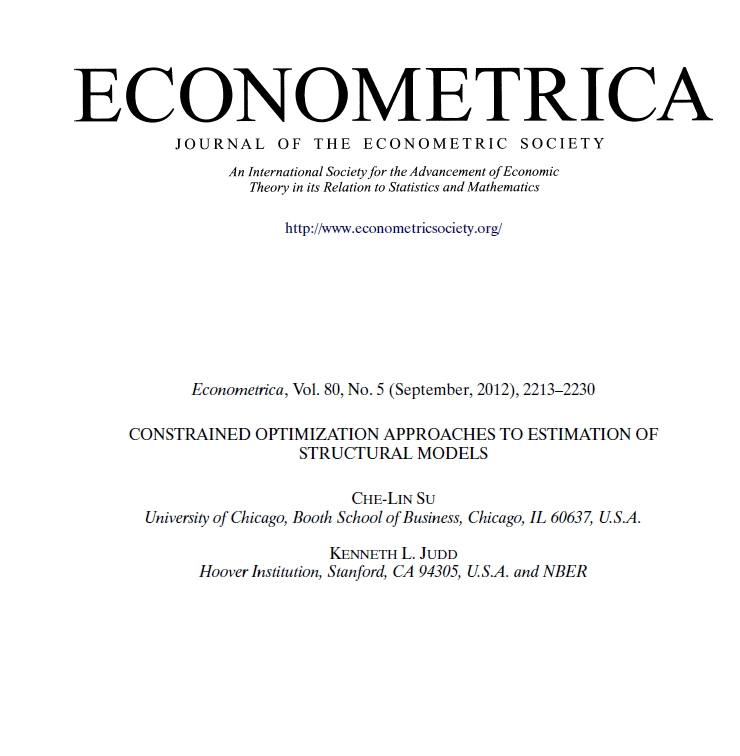
\includegraphics[width=0.6\textwidth]{Su_Judd_2012_Ecta_cover.jpg}
\end{frame}

\begin{frame}
MPEC in the Rust bus engine problem
\bigskip{}
\begin{itemize}
\itemsep1.5em
\item<2-> Compare MPEC with NFXP in the Rust (1987) model
\item<3-> Su \& Judd (2012) initially reported substantial speed improvements
\item<4-> \textcolor{navy}{However:} Iskhakov et al. (2016) showed similar performance when both methods are properly optimized
\item<5-> Key advantages of MPEC: ease of implementation and robustness
\item<6-> The optimizer sees constraints and makes ``smarter'' guesses
\end{itemize}
\end{frame}

\begin{frame}

MPEC example: Cournot oligopoly

\bigskip{}

\begin{itemize}
\itemsep1.5em
\item<2-> JuMP, with an add-on package Complementarity.jl, supports MPEC
\item<3-> Example: $N$-firm symmetric Cournot monopolistic competition
\item<4-> Each firm $i$ chooses output $q_i$ to maximize profit, subject to $q_{-i}$
\item<5-> Marginal cost $c_i$ is assumed to be constant and equal across all firms
\item<6-> Market demand is given by $P(Q) = a - bQ$
\end{itemize}

\end{frame}

\begin{frame}

This problem is easy to solve analytically:

\bigskip{}

\onslide<2->{
\begin{align*}
q^* &= \frac{a-c}{b(N+1)}\\
\\
P^* &= \frac{a+Nc}{N+1}
\end{align*}
}

\end{frame}

\begin{frame}

Cournot oligopoly using JuMP

\bigskip{}

\begin{itemize}
\itemsep1.5em
\item<2-> JuMP allows us to formulate this as an MPEC problem
\item<3-> Firm 1 minimizes negative profit subject to other firms' FOCs
\item<4-> We impose symmetry: all firms choose the same output in equilibrium
\item<5-> The optimizer finds the equilibrium without nested fixed-point iteration
\end{itemize}

\end{frame}


\begin{frame}

We can easily extend the model:

\bigskip{}

\begin{itemize}
\itemsep1.5em
\item<2-> Add capacity constraints: $0 \leq q_i \leq L$
\item<3-> Vary the number of firms $N$
\item<4-> Allow asymmetric costs $c_i$
\item<5-> Use non-linear demand functions
\end{itemize}

\end{frame}

\end{document}